\chapter{训练深度模型的优化方法}
\label{chap:8}
%%%%%%%%%%%%%%%%%%%%%%%%%%%%%%%%%%%%%%%%%%%%%%%%%%%%%%%%%
%%%%%%%%%%%%%%%%%%% author:wzwei1636@163.com  %%%%%%%%%%%
%%%%%%%%%%%%%%%%%%% part:8.0-8.2              %%%%%%%%%%%
%%%%%%%%%%%%%%%%%%%%%%%%%%%%%%%%%%%%%%%%%%%%%%%%%%%%%%%%%
\section{8.0}


深度学习算法在许多场景下涉及到最优化。例如,在PCA模型的性能推断上涉及解决一个最优化问题。我们经常用最优化解析方法去证明或者设计算法。在深度学习包含的所有最优化问题中,最困难的是神经网络训练。甚至https://preview.overleaf.com/public/yqhdxhwbpfpr/images/da8c750f57110730fbd2f2805ecef1d164d8f7d3.jpeg为了解决神经网络训练的一个实例,花费几天或者上月的时间在几百台机器上都是很常见的,因为这个问题非常重要且代价很大,然而我们已经开发了一类特殊的最优化技术去解决它。本章将给出训练神经网络的最优化技术。

如果你不熟悉基于梯度的最优化方法的基本理论,我们推荐复习第四章。那一章包含简短的数值最优化方法的概述。

本章集中于一个特殊的最优化场景,找到能够显著减少神经网络损失函数$J(\theta)$的参数$\theta$,通常包含在整个训练集评估的性能度量以及额外的正则化项。

刚开始,我们将描述对于一个机器学习任务,在训练算法上使用的最优化方法有别于纯粹的最优化。下一步,我们将给出一些具体的优化神经网络的难点。然后定义一些实践上的算法,包含最优化算法本身和初始化参数的一些策略。更加高级的算法在训练或者利用包含在损失函数的二阶导数来调整学习率。最后,通过回顾一系列的优化策略,我们可以将一些简单的最优化算法结合转化为更高层次的程序。

\section{学习和优化有什么不同}

训练深度模型中使用的最优化算法在某些方面不同于传统的最优化算法。机器学习经常表现的间接。在大部分机器学习的场景中,我们关注性能度量$P$,它是在测试集中定义的,也是非常棘手的。我们仅仅间接优化P,我们希望通过减少损失函数$J(\Vtheta)$提升性能$P$。相比之下,纯粹的最优化方法,其目的在于最小化$J(\Vtheta)$。训练深度模型的最优化算法通常也包括在机器学习目标函数的特殊结构上的一些特性。

通常,损失函数可写为训练集上的平均,如

\begin{equation}
J(\theta)=E_{(x,y)\thicksim\hat{P}_{data}}L(f(x;\theta),y)
\end{equation}

其中L是每个样本的损失函数,当输入为x,$f(x;\theta)$是预测的输出值,$\hat{p}_{data}$在监督学习中,y是目标值。整个这章,我们开发非正则化监督例子,其中对于L,参数是$f(x;\theta)$和y。然而,很轻易去扩展,例如,为了开发正则化的各种形式或非监督学习,在参数中包含$\theta$或x,排除y。

等式8.1定义了一个关于训练集的目标函数。我们通常对相应的目标函数最小化,其中期望 是在数据的生成分布$P_{data}$而不是有限的训练集上。

\begin{equation}
J^*(\theta)=E_{(x,y)\thicksim\hat{P}_{data}}L(f(x;\theta),y)
\end{equation}

\subsection{经验风险最小化}

机器学习算法的目标是在等式减小泛化误差,即所谓的风险。需要强调的是期望是取值在真实潜在分布$p_{data}$上的。如果我们知道真实分布$P_{data}(x,y)$,风险最小化将由最优化算法解决。然而,当我们不知道$P_{data}(x,y)$,仅仅有一些训练样本时,就遇到了一个机器学习问题。

最简单的方式是将机器学习问题转化为最优化问题,通过在训练集上最小化期望损失。也就意味着用经验分布$\hat{P}(x,y)$替换真实分布p(x,y)。最小化经验风险:

\begin{equation}
E_{(x,y)\thicksim\hat{P}_{data}}[L(f(x;\theta),y)]=\frac{1}{m}\sum_{i=1}^mL(f(x^{(i)};\theta),y^{(i)})
\end{equation}

其中m是训练样本的个数。

基于最小化平均训练误差的训练过程即为经验风险最小化。并不是直接优化风险,我们最优化经验风险,希望经验风险显著减小。基于不同的条件各种理论结果建立起来了,真实的风险是可以通过不同的变量减小。

然后,最小化经验风险易于过拟合。在许多情况下,最小化经验风险并不真正可行。大部分有效的模型最优化算法是基于梯度下降的,然而许多有用的损失函数,例如0-1损失函数,没有导数。这里两个问题意味着,在深度学习中,我们很难最小化经验损失。相反,我们必须使用略有不同的方法,我们真正优化的量甚至不同于我们真实想要优化的量。

\subsection{替化损失函数和提前终止}

有时,损失函数我们真正关心的(分类误差)并不是有效的优化。例如,严格最小化期望0-1损失函数明显棘手的(在维数上是指数的),甚至是对于一个线性分类器(Marcotte and Savard, 1992).在这种情况下,一个典型的优化是用代理损失函数替代,充当一个代理但是却非常有效。例如,正例的非负对数似然就是替代0-1损失的。非负对数似然允许模型估计类别的条件概率。给定输入,若模型确实有效,则选择最小期望分类误差。

在某些情况下,一个代理损失函数事实上导致可以学到更多。例如,当训练中用对数似然替代时,当训练集上0-1损失函数为0时,在测试集上0-1损失函数通常连续减少。这是因为尽管0-1损失是0,我们可以提高分类器的鲁棒性进一步的区分不同的类,获取更可靠的分类器,因此相比于在训练集上简单的最小化平均0-1损失,能获取更多的信息。

一般的最优化方法和深度学习中的最优化算法的一个重要差异在于,我们在使用训练算法时,通常不会再局部最小值停止。相反,当基于提前停止的收敛规则满足时,一个机器学习算法通常最小化一个代理损失函数停止。典型的,提前停止规则是基于真实的潜在的损失函数,例如在验证集上度量的0-1损失,当过拟合开始发生时,算法停止。尽管替代的损失函数依然有比较大的导数,训练能停止。这非常不同于纯粹的最优化方法,其中最优化算法当梯度非常小时,被认为是收敛的。

\subsection{批算法和小批算法}

机器学习算法不同于一般的最优化算法的一个方面在于为目标函数在训练集上被分解为为训练样本上的求和。机器学习优化算法通常使用整个损失函数中的一部分项去更新基于估计损失函数的期望值。
例如,在对数空间中,极大似然估计问题可以分解成每个样本的和:

\begin{equation}
\theta_{ML}=argmax_\theta\sum_{i=1}^m log p_{model}(x^{(i)},y^{(i)};\theta)
\end{equation}

最大化此项等价于最大化定义在训练集上的经验分布的期望:

\begin{equation}
J(\theta)=E_{(x,y)\thicksim\hat{P}_{data}} log p_{model}(x,y;\theta)
\end{equation}

目标函数的多数性质被大部分最优化算法所使用的也是训练集上的期望。例如,通常大部分使用的性质是梯度:

\begin{equation}
\nabla_{\theta}J(\theta)=E_{(x,y)\thicksim\hat{P}_{data}}\nabla_{\theta} log p_{model}(x,y;\theta)
\end{equation}

准确计算这个期望代价非常大,因为它需要在整个数据集的每个实例上评估模型。实践中,我们通过对数据集进行随机抽样来计算这些期望,然后再在实例上取均值。
    
回忆n个样本均值的标准差$\frac{\sigma}{\sqrt{n}}$,其中$\sigma$是这些样本的标准差。在100个实例和1000个实例上比较梯度的两个假设估计,后者比前者需要多出100倍的计算,但是平均能减少10倍的标准差。大多数的最优化算法当他们能快速近似计算梯度时往往比缓慢计算的严格梯度要收敛的更快。

其他有助于来自小样本的梯度统计估计在训练样本集上是多余的,最糟糕的情况,训练集中的所有m个样本,是彼此相同的。一个基于抽样的梯度估计通过m个样本能正确计算,比使用朴素方法计算次数要少。实践中,我们不可能遇到这种情况,但是我们可以使用大样本量计算梯度。

最优化算法使用整个训练集称之为批或确定梯度方法,因为它们通过一个大的批次同时计算所有的样本量。这个术语可能与 “batch”有点混淆,其经常被使用其描述由最小批处理随机梯度下降的分批处理,典型的,术语批随机梯度下降暗含着真个训练集的使用,同时术语batch的使用并不是描述着一组样本。例如,通常使用术语“bitch size”描绘批梯度的规模。

最优化算法有时一次使用一个实例称之为随机或者在线方法。术语在线有时被保留的情况下来自于,从一个不断创建的例子,而不是传输固定大小的训练集。

深度学习使用的大部分算法介于两者之间,即使用一个以上或者少于所以的训练样本。传统上被称之为批处理或者批处理随机方法,现在统一简称为随机方法。

随机方法的标准范例是随机梯度下降,在8.3.1会详细说明。

批规模由下面几个因素驱动:
1.更大的批次提供一个更加精确的梯度估计,但是不是呈线性的返回。
2.在极小的批次下,多核架构一般未被充分利用,这个激发使用一些绝对数量的最小批次,在处理一个批上时间上并没有减少。
3.如果批次中所有的示例被并行处理,则大量的内存被批规模消耗掉。许多硬件限制了批的规模。
4.各种硬件通过使用特定的数组可以获得更好的运行,特别是在使用GPUs的过程中,2次幂的批规模来提供更好的性能。明显的2的幂次方的批规模从32变化到256,为了尝试大的模型,可能是16.
5.小批次可能提供一个正则化的影响,可能因为噪声被被添加到学习过程,泛化误差对于规模为1的批次是最好的。在这个规模上进行训练可能需要小的学习速率来维持因为在梯度估计中的高方差。总的运行时间可能非常高因为需要采取更多的步数,均是因为学习速率的减小和需要采取更多的步数来观测整个训练集。

不同的算法通过不同的方式使用最小批的各种信息。一些算法对样本误差非常敏感,可能是因为他们使用非常少的样本取估计准确度,或者是因为他们放大样本误差。仅仅基于梯度g计算更新通常相对健壮,他们可以处理如100的批规模。二阶方法,通过使用Hessian矩阵H,通过计算$H^{-1}g$进行更新,典型的需要如10000的更大的批次。这些大的批次规模需要最小化估计$H^{-1}g$的波动。设想H使用非常少的条件数被完美估计。乘以H或者它的逆放大预先存在的错误,这种情况下,在g中存在估计误差,估计g中非常小的变化能引起更新$H^{-1}g$的巨大变化,甚至当H被完美估计。当然H只能被近似估计,因此更新$H^{-1}g$将比我们通过应用少量的条件去估计g来预测会包含更多的错误。

最小批被随机选择是非常重要的,计算样本的期望梯度的无偏估计需要样本是独立的,我们也希望两个随后的梯度估计是相互独立的,我们希望两个随后的梯度估计相互独立,许多数据集一般被设计成许多连续的例子是高度相关的。例如,我们可能有一系列的关于血液样本的医药数据。对第一个病人,在不同时间获取5例血液样本,然后从第二个病人那里获取3例血液样本,然后依次进行这样的操作,如果我们按照顺序从中取出实例,则每个minibatches将是极度有偏的,因为它将代表数据集中许多患者的最显著的那个。在这种情况下,数据集中实例的顺序将有重要意义,因为必须在选择minibatches之前必须打乱实例的顺序。对于大数据集而言,例如一个数据中心包含几十亿的实例,每次随机抽样取构造

minibatches是不现实的。幸运的是,实践上足够去打乱实例的顺序,并以无序的形式存储。这将强加一个固定连续的minibatches,从而在所有的模型训练中使用,当使用整个数据集时,每一个单独的模型将被迫重用这个排序。然而,来自真正随机选择的偏差看起来并没有一个显著的有害影响。不打乱实例的顺序将严重减弱算法的有效性。

机器学习中的许多最优化问题可以在训练集中进行分解,从而我们可以并行的不同的实例上计算整个单独的更新。换言之,我们可以计算更新能够同时对于每个X的minibatch最小化J(x),从而对多个minibatch计算更新。这些异步并行分布式方法在12.1.3将被讨论。

一个有趣的动机对于minibatch随机梯度下降在于只要没有实例被重复,将一直会有泛化误差的梯度。大多数minibatch随机梯度下降方法的实现会打乱数据顺序一次,然后多次遍历数据更新参数。第一次遍历时,每个minibatch样本都用来计算真实泛化误差的无偏估计。第二次遍历时,此时已经是有偏估计了,因为使用了由重新采样生成的值,而不是从数据的生成分布上获取新的样本。	

事实上随机梯度下降最小化泛化误差是在线学习最简单的情况,其中样本或者minibatch都是从数据流中抽取出来的。换句话说,并不是接收固定数量的训练集,学习其类似于生物能够在每个瞬间了解新的实例,其中每个样本(x,y)来自于生成分布$P_{data}(x,y)$。在这种情况下,实例不会重复,每个经验来自$P_{data}$都是公平的。

当x和y都是离散时,相等最易得到。此时,泛化误差被记为:

\begin{equation}
J^*(\theta)=\sum_x\sum_yp_{data}(x,y)L(f(x;\theta),y)
\end{equation}

以及梯度为:

\begin{equation}
g=\nabla_{\theta}J^*(\theta)=\sum_x\sum_yp_{data}(x,y)\nabla_{\theta}L(f(x;\theta),y)
\end{equation}

我们已经了解了等式8.5和8.6的对数似然的情况,对于除似然之外的其他函数L也是成立的。当x和y是连续的,关于$P_{data}$和L的一些假设,一个类似的结果也可以得到。

因此,通过对来自生成分布$P_{data}$的实例$\{X^{(1)},\dots X^{(m)}\}$和响应变量$y^i$进行抽样,我们就可以获取泛化误差梯度的无偏估计。计算关于参数的损失梯度:

\begin{equation}
\hat{g}=\frac{1}{m}\nabla_{\theta}\sum_iL(f(x^{(i)};\theta),y^{(i)})
\end{equation}

在泛化误差上通过沿着$\hat{g}$的方向上执行SGD来更新theta。

当然,这个理解仅适用于当实例不被重新使用时。最好是多次使用训练集,除非训练集特别大。当多次训练时,只有第一次训练泛化误差的梯度是无偏的,当然了,其他的训练足够有效,因为通过增加训练误差和测试误差之间的差距来减小训练误差,因此来抵消。

随着数据规模的快速扩大,对于机器学习应用去一次使用一个实例,甚至使用不完整的训练集,正变得越来越寻常。当使用特别大的训练集时,过拟合不是一个问题,因此欠你和和计算有效性变成了主要担忧的事情。具体可参考Bottou and Bousquet(2008)关于随着训练集规模的增长,关于在计算泛化误差上的瓶颈的讨论。

\section{神经网络最优化算法的挑战}

一般上最优化算法都是一个非常困难的工作。过去机器学习通过仔细设计目标函数和约束条件来避免常规的优化难度,以此来确保最优化问题是凸优化。当训练神经网络时,我们必须面对一般的非凸问题。在这一部分,我们总结了一些对于训练深度模型所涉及的最优化问题的显著的困难和挑战。

\subsection{病态}

当优化凸函数时,会引起一些挑战。其中最突出的就是黑塞矩阵H的病态问题。这在大多数数值最优化中是一个非常普遍的问题,凸或非凸在4.3.1有详细的描述。
	病态问题一般认为是存在于神经网络训练的问题。病态会引起SGD“卡住”也就是说甚至非常小的步长都会引起损失函数的急剧增加。
	回忆等式4.9,损失函数的二阶泰勒级数展开预测梯度减少  的步长将会给损失函数增加

\begin{equation}
\frac{1}{2} \varepsilon^2 g^THg-\varepsilon g^Tg
\end{equation}

当$\frac{1}{2} \varepsilon^2 g^THg$超出$\varepsilon g^Tg$,将会引发梯度的病态。

% \begin{figure}[htbp]
%    \centering
%    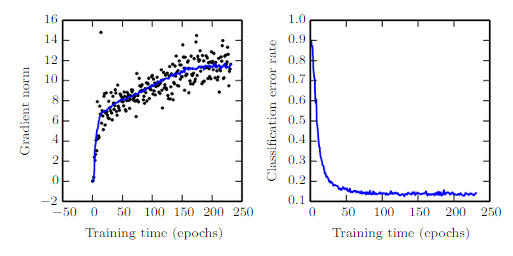
\includegraphics[width=6in]{fig/chap8/8_1.png} 
%    \caption{}
%    \label{fig:8.1}
% \end{figure}

为了判定病态是否对于神经网络的训练不利,通过监控$g^Tg$和$g^THg$的平方梯度。在许多情况下,梯度范数在学习时并不会明显减少,但是$g^THg$会数量级的增加。结果就是学习变得非常慢,尽管存在一个强大的梯度,但是因为学习率必须缩小以弥补更强曲率。图8.1展示了在成功训练神经网络梯度显著增加的例子。

尽管病态在除神经网络训练之外也会出现在其他情况下,但是一些技术已经用于实践,在许多场景下也非常少应用于神经网络。例如,牛顿法对于没有什么条件的Hessian矩阵,最小化凸函数是一个非常优秀的工具,但是在后面的部分,我们将说明牛顿法在它应用到神经网络之前需要重要的修正。

\subsection{局部极小值}

一个凸优化问题的最显著问题之一就是会找到局部最小值问题。任何局部最小值确保是一个全局最小值。一些凸优化函数在底部有一个平坦的区域而不是单个的全局最小值点,因此这个平坦区域的任何一个点都可以被视为一个可行解。当优化一个凸函数时,如果我们发现任何形式的临界点,那么我们就找到了一个好的解决方法。

对于非凸函数,例如神经网络,可能有许多的局部最小值。事实上,任何一个深度模型本质上都确保有一个非常大的局部最优解。然而,正如我们将要看到的,这将不是一个主要的问题。

神经网络和多个等效参数化的潜在模型都有多个局部极小的模型识别问题。一个模型被认为是可识别的,如果一个足够大的训练集可以排除所有除模型参数的设置。含有潜在变量的模型经常是不可识别的,因为我们可以变换潜在变量获取等价的模型。例如,我们可以取神经网络,修改第一层通过将神经元i的输入权重变量和神经元j的输入权重变量交换,输出了相同的权重向量。如果我们有m层,每一层有n个神经元,则将有$n!^{m}$种方式设计隐藏的神经元。这种非识别称之为重空间对称性。

除了重空间对称性,各种神经网络有其他引起不可识别的因素。例如,在任何修正线性或maxout网络,我们如果能度量所有的输出权重,那么可以度量所有的输入权重和单位偏差$\alpha$,意味着如果损失函数不包含例如权重衰减的项,直接基于权重而不是模型的输出——修正线性或maxout网络的每一个局部最小值位于(m*n)维的等价局部最小值的超平面。

这些模型的可识别问题意味着神经网络的损失函数中有特别大或者不可数的局部最小值。然而,由不可识别引起的所有局部最小值都等价于损失函数的的其他值。因此,这些局部最小值不是一个有问题的非凸形式。

如果局部最小值与全局最小值比较有高的代价损失,则局部最小值是有问题的。甚至在没有隐藏神经元的情况下构造一个小的神经网络,局部最小值的代价损失要比全局最小值要高(Sontag and Sussman, 1989; Brady et al., 1989; Gori and Tesi, 1992).若局部最小值有很高的代价损失且较常见,则对于基于梯度的最优化算法来说就是一个严重的问题。

对于在神经网络的实践中是否有代价损失较高的许多局部最小值,且是否最优化算法会遇到这个问题,这依然是一个开放问题。多年来,大多数的实践者相信局部最小值是困扰神经网络最优化的常见问题。现在,似乎并不是这样,这个问题仍然是研究的热门领域,但是许多专家怀疑对于足够大的神经网络,大部分的局部最小值有较小的代价损失值,去找到一个真正的全局最小值并不是很重要,宁愿在参数空间找到一个点有较小的代价损失而不是最小的代价损失。(Saxe et al., 2013; Dauphin et al., 2014; Goodfellow et al., 2015; Choromanska et al., 2014).

许多实践者将神经网络最优化中遇到的困难都归咎于局部最小值。我们鼓励实践者仔细的去测试具体问题。一个测试可以通过不断计算梯度的范数来排除局部最小值问题。如果梯度的范数并不显著减少,这个问题既不是局部最小值也不是其他类型的临界值。这种负检验可以消除局部最小值。在高维空间,明确确定局部最小值是非常困难的问题。

\subsection{高原,鞍点和平台}

对于许多高维非凸函数,局部最小或最大事实上与另外一种比较罕见的鞍点,都是梯度为0的情况。鞍点周围的点比其他点有更大的损失。在鞍点,黑塞矩阵既有整的特征值也有负的特征值。与正的特征值相关的特征向量比鞍点有更大的损失,而接近负特征值的特征向量有着更小的损失。我们可以将鞍点视为沿着损失函数某一横截面的一个局部最小值,以及损失函数另一横截面的一个局部最大值。图4.5说明了这个方面。

许多不同类别的随机函数表现出如下的行为:在低维空间,局部最小值很常见。在高维空间,局部最小值罕见,而鞍点非常常见。对于函数$f:\square^n\to \square$ ,鞍点的数量相比局部最小值随着n的增加呈现指数增长。为了直观理解这个现象,观测Heassian矩阵在局部最小值点只有正的特征值。而Hessian矩阵在鞍点既有正的又有负的特征值。想象一下,每一个特征值的符号是通过翻转一个硬币而产生的。在一维的情况下,通过投掷硬币得到正面是很容易获得一个局部极小值。在n维空间,所有n个硬币都是正面的概率呈现负指数的情况。
见Dauphin et al. (2014),回顾相关的理论工作。

许多随机函数令人惊讶的性质在于当位于代价较低的区域时,Hessian矩阵的特征值更可能是正的,类以硬币投掷,意味着如果我们在某个重要的点有着较低的损失,则硬币可能n次朝上。也意味着局部最小值更有能有更小的损失。临界点上有着更高的代价损失意味着很可能是鞍点,临界点上有点特别高的代价损失意味着很可能是局部最小值。

这种现象发生在许多不同类别的随机函数上。神经网络也会遇到这种情况吗?Baldi and Hornik (1989)理论上证明了没有非线性的浅自动编码器(前馈神经网络被训练使得输入和输出保持一致,第14章有相关说明)有全局最小值和鞍点,此外没有局部最小值比全局最小值有更高的代价损失。没有证明观测到这些结果延伸到没有非线性的深度神经网络,这些网络的输出是输入的线性函数,但是学习一个非线性神经网络模型是很有用的,因为它们的损失函数是关于参数的非凸函数。这些网络本质上仅仅是多个矩阵结合在一起。Saxe et al. (2013) 提供准确的解决方案,在这样的网络中完成动态学习,也展示了学习这些模型可以获取到在用非线性激活函数训练深度模型观测到的许多定性特征。Dauphin et al. (2014)实验上展示了真正的神经网络也有包含许多较高损失代价鞍点的损失函数。Choromanska et al. (2014)提供了额外的理论论证,证明了与神经网络相关的其他类型的高维随机函数也是如此。

对于训练算法中鞍点带来的影响是什么?对于仅仅使用梯度信息的一阶最优化算法,这种情形不是特别清晰。靠近鞍点,梯度经常变得非常小。另外一方面,梯度下降经验上看上去在许多情况下可以摆脱鞍点。Goodfellow et al. (2015) 提供了一些先进的神经网络的路径图的可视化,图8.2就是一个例子展示。这些直观上表明了靠近比较突出的鞍点损失函数平坦且权重为0,但是它们也表明梯度下降轨迹会迅速逃离这个区域。Goodfellow et al. (2015)也论证了连续时间梯度下降靠近鞍点是排斥而不是吸引,但是这种情况与许多现实中使用的梯度下降可能有许多不同。

% \begin{figure}[htbp]
%    \centering
%    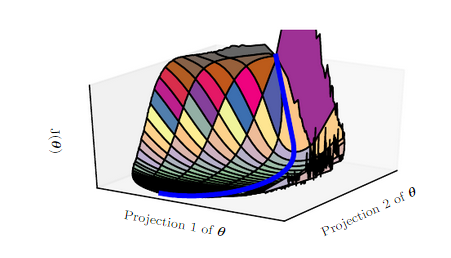
\includegraphics[width=6in]{fig/chap8/8_2.png} 
%    \caption{}
%    \label{fig:8.2}
% \end{figure}

对于牛顿法,很明显鞍点构成一个问题。梯度下降被设计成是下山,并不明显是寻找一个临界点。牛顿法被设计解决某个点的梯度为0。没有合适的修改,它将落入鞍点,在高维空间中鞍点的扩散可以解释为什么二阶方法对于神经网络训练为什么没有成功取代梯度下降。Dauphin et al. (2014)引入对于二阶最优化算法的无鞍牛顿法,展示了比传统的方法显著提高。二阶方法对于度量庞大的神经网络依然非常困难,但是如果可以度量,这个无鞍的解决方法还是有很多前景的。

除了最小值和鞍点还有其他类型梯度为0的点,也有极大值,和鞍点一样来自最优化问题,许多算法并不对极大值感兴趣,除了未修改的牛顿法。

也有许多常数对应的平坦区域。在这些点,梯度和Hessian矩阵都是0.这些退化的点对于所有的数值最优化算法都是很大的问题。在凸优化问题中,一个宽且平坦的区域一定会包含所有的全局最小值,但是在一般的最优化问题中,这样的区域对应目标函数的一个比较大的值。

\subsection{悬崖和梯度爆炸}

含有多层的神经网络经常会有非常陡峭的区域类似悬崖,图8.3进行了说明。这些结果来自于许多大的权重值相乘。在面对一个非常陡峭的悬崖结构时,梯度更新随着参数的变化会移动的非常远,通常会调离悬崖结构。

% \begin{figure}[htbp]
%    \centering
%    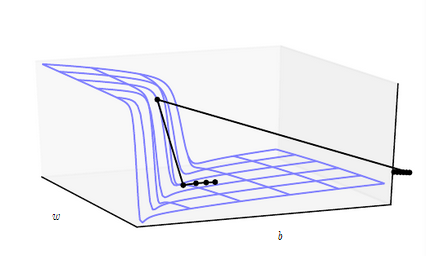
\includegraphics[width=6in]{fig/chap8/8_3.png} 
%    \caption{}
%    \label{fig:8.3}
% \end{figure}

这个悬崖是非常危险的,无论我们从上面或是下面接近它,但是幸运的是通过使用缩短梯度可以避免这些严重的后果。基本思想是:回忆梯度并没有指定最优步长,但只是沿着在极度小的区域中的最优方向。当传统的梯度下降算法采取大的步长时,启发式的缩短梯度会干预使得步长的减小足够小,从而不太可能落在梯度沿着最速下降的方向以外的区域。悬崖结构对于递归神经网络是非常常见的,因为这些模型设计带许多因数的相乘,长时间序列因此因为乘法产生了一个极端值。

\subsection{长期依赖}

神经网络最优化算法的另外一个困难必须克服是由当计算图变得非常深时引起的。含有多层的前馈神经网络或有如此神的计算图,递归神经网络也是如此,第10章会有描述,通过一个长的时间序列上每隔一个时间段重复应用相同的操作会构造出深的计算图。重复使用相同的参数会引起明显的困难。

例如,设想一个计算图包含重复乘以W的步骤。t步之后,等价于乘以$W^t$。设想W有特征分解$W=Vdiag(\lambda)V^{-1}$。这种简单的情况下,可以直接看到如下:

\begin{equation}
W^t=(V_{diag}(\lambda)V^{-1})^t=V_{diag}(\lambda)^tV^{(-1)}
\end{equation}

任何特征值$\lambda_i$当大于1时,量级会指数扩张,当小于1时,会减小趋近于0.这个消失和梯度爆炸问题涉及到事实上图是根据$diag(\lambda)^t$度量的。梯度消失对于从哪些参数方面去改善损失函数是非常困难的,而梯度爆炸使得学习不稳定。悬崖结构早期描述了促进缩短梯度是梯度爆炸的示例。

每次重复乘以W类似于使用幂算法去找到矩阵W的最大特征值以及相应的特征向量。从这一点看来将并不奇怪,$x^TW^t$将最终舍弃所有的正定于W的特征向量的x。

递归神经网络每次使用同一个W,但是前馈神经网络不是,因此尽管非常深的前馈神经网络可以在很多程度上避免梯度消失和爆炸问题(Sussillo, 2014).

我们将推迟关于训练递归神经网络挑战的讨论,知道10.7部分,在那里递归神经网络将更详细的被描述。

\subsection{不精确梯度}

大多数优化算法都需要提取梯度或者Hessian矩阵,而现实中我们通常只能使用带噪声或有偏来估计这些量。几乎每个深度学习算法都依赖于基于采样的估计,至少使用训练样本的最小批次来计算梯度。

在其他情况下,我们想要最小化目标函数实际上是无解的。当目标函数无解时,通常梯度也是无法计算的。这些问题大多出现在第三部分中更高级的模型中。例如对比散度给出近似比较难解的玻尔兹曼机的极大似然的梯度技术。

各种神经网络最优化算法被设计去解释梯度估计上的缺陷。通过选择替代的损失函数可以避免这个问题。

\subsection{局部和全局结构的不一致性}

迄今为止我们讨论的许多问题对应于损失函数在单点的性质——如果$J(\theta)$在$\theta$处没有约束或者是$\theta$位于悬崖,又或者是$\theta$是一个鞍点,是很难取一个步长的。

克服在单点的上述问题,以及依然表现不佳,如果导致局部最大改善的方向不是朝着许多更小代价损失的区域方向,是有可能的。

Goodfellow et al. (2015)论证了训练过程的运行时间是归结于到达解决方法的轨迹长度。图8.2证明了学习轨迹花费的大部分时间是在追踪围绕山地结构的很宽的弧线。

许多关于最优化问题研究的困难集中于是否训练会到达全局最小值、局部极小值、鞍点。但是实践中神经网络不会到达任何类型的临界点,图8.1表明了神经网络不会落在小梯度的区域。事实上,这些临界点甚至没有必要存在。例如损失函数$-logp(y|x;\theta)$没有全局最小值点,相反可以渐进到一些值,此时模型也会更加准确。对于离散y和$p(y|x;\theta)$由softmax提供的分类器,非负对数似然当模型可以正确对训练集中的每个示例正确分类时,可以沿任意方向趋于0,但是不可能严格等于0.同样的,真实模型$p(y|x;\theta)=N(y;f(\theta,\beta^{-1}))$有负对数似然渐进于负无穷,若$f(\theta)$可以正确预测训练集中的目标y,学习算法将无限增加增加$\beta$。图8.4说明了局部最优化失败去寻找一个好的损失函数,即使是存在任何的局部极小值或者鞍点。

未来的研究需要进一步理解影响学习轨迹长度和更好描述结果的因素。

% \begin{figure}[htbp]
%    \centering
%    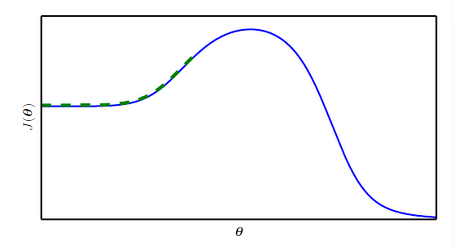
\includegraphics[width=6in]{fig/chap8/8_4.png} 
%    \caption{}
%    \label{fig:8.4}
% \end{figure}

许多当前的研究方向旨在对于复杂全局结果找到好的初始点,而不是使用非局部移动开发算法。

梯度下降和所有的学习算法对于基于通过较小、局部的移动来训练神经网络是有效的。先前的部分主要集中于这些局部移动的正确方向将非常困难去计算。可以计算这些目标函数的梯度,近似通过偏差或者方差沿着估计的正确方向近似。目标函数缺少约束条件或不连续的梯度,将导致区域非常小。在这些情况下,步长大小为$\varepsilon$的局部下降可以定义一个合理的短路径的解决方案,但我们只能够计算步长大小为$\delta\square\varepsilon$的局部下降。局部下降可能或不可能定义一个解决方案,但路径包含许多步骤,所以这些路径会引发高的计算成本。当函数有一个基表大的平坦区域时或者设法到达临界点时,局部信息没有作用。其他情况,拒不移动太贪婪将导致远离任何解,如图8.4,或者沿着解的多余的长轨迹,如图8.2.当前我们不了解这些问题对于引起神经网络优化困难,哪些是最相关的,这是一个热门的研究领域。

无论哪个问题都是非常重要的,如果存在一个区域连接相应局部下降解的路径,或者如果我们使用比较好的区域初始化学习 。最后的观点建议为传统的最优化算法研究选择好的初始点。

\subsection{理论上的优化限制}

一些理论结果表明为神经网络设计的最优化算法会有性能上的限制(Blum and Rivest,
1992; Judd, 1989; Wolpert and MacReady, 1997)。通常这些结果在实践中神经网络的使用上是不可用的。

一些理论结果只适用于神经网络的单元输出离散值。但是大多数神经网络单元输出都睡平滑的值,使得通过局部搜索的优化可行。一些理论结果表明存在一些有问题的类是难以被正确分类的,但是很难讲清楚是否存在一个特定的问题导致错误分类。其他的一些结果表明为一个特定大小的网络找到solution是很棘手的,但是在实践中我们可以简单地找出一个solution,通过使用一个较大的网络设定较多的参数,得到一个可以接受的solution。而且在神经网络训练中,通常不关心找到一个函数的严格最小值,而是在于足够去减少它的泛化误差。理论分析一个优化算法是否能完成是相当困难的,因此在机器学习研究中药更加注重优化算法的性能的现实结果














\section{训练深度模型的优化方法}

深度学习算法在许多场景下涉及到最优化。例如,在PCA模型的性能推断上涉及解决一个最优化问题。我们经常用最优化解析方法去证明或者设计算法。在深度学习包含的所有最优化问题中,最困难的是神经网络训练。甚至为了解决神经网络训练的一个实例,花费几天或者上月的时间在几百台机器上都是很常见的,因为这个问题非常重要且代价很大,然而我们已经开发了一类特殊的最优化技术去解决它。本章将给出训练神经网络的最优化技术。

如果你不熟悉基于梯度的最优化方法的基本理论,我们推荐复习第四章。那一章包含简短的数值最优化方法的概述。

本章集中于一个特殊的最优化场景,找到能够显著减少神经网络损失函数$J(\Vtheta)$的参数$\Vtheta$,通常包含在整个训练集评估的性能度量以及额外的正则化项。
	
刚开始,我们将描述对于一个机器学习任务,在训练算法上使用的最优化方法有别于纯粹的最优化。下一步,我们将给出一些具体的优化神经网络的难点。然后定义一些实践上的算法,包含最优化算法本身和初始化参数的一些策略。更加高级的算法在训练或者利用包含在损失函数的二阶导数来调整学习率。最后,通过回顾一系列的优化策略,我们可以将一些简单的最优化算法结合转化为更高层次的程序。

\section{学习和优化有什么不同}

训练深度模型中使用的最优化算法在某些方面不同于传统的最优化算法。机器学习经常表现的间接。在大部分机器学习的场景中,我们关注性能度量$P$.,它是在测试集中定义的,也是非常棘手的。我们仅仅间接优化$P$.,我们希望通过减少损失函数$J(\Vtheta)$提升性能$P$。相比之下,纯粹的最优化方法,其目的在于最小化$J(\Vtheta)$。训练深度模型的最优化算法通常也包括在机器学习目标函数的特殊结构上的一些特性。

通常,损失函数可写为训练集上的平均,如
\begin{equation}
\label{eq:8.1}
    J(\Vtheta) = \SetE_{(\RVx, \RSy) \sim\hat{p}_\text{data}} L(f(\Vx ; \Vtheta), y),
\end{equation}
其中$L$是每个样本的损失函数,$f(\Vx;\Vtheta)$是输入是$\Vx$时的预测输出,$\hat{p}_{\text{data}}$是经验分布。
监督学习中,$y$是目标输出。
在本章中,我们会介绍不带正则项的监督学习,$L$的参数是$f(\Vx;\Vtheta)$和$y$。
很容易将这种监督学习扩展成其他形式,如为了开发正则化的各种形式或非监督学习,在参数中包含$\Vtheta$或者$\Vx$,排除参数$y$。

eqnref{eq:8.1} 定义了训练集上的目标函数。我们通常对相应的目标函数最小化,其中期望是在数据的生成分布$p_{\text{data}}$而不是有限的训练集。
\begin{equation}
\label{eq:8.2}
    J^*(\Vtheta) = \SetE_{(\RVx, \RSy) \sim p_\text{data}} L(f(\Vx ;\Vtheta),y).
\end{equation}

\subsection{经验风险最小化}

机器学习算法的目标是在(公式引用出错)减小泛化误差,即所谓的风险。需要强调的是期望是取值在真实潜在分布$p_\text{data}$上的。如果我们知道真实分布$p_\text{data}(\Vx, y)$,风险最小化将由最优化算法解决。然而,当我们不知道$p_\text{data}(\Vx, y)$,仅仅有一些训练样本时,就遇到了一个机器学习问题。

最简单的方式是将机器学习问题转化为最优化问题,通过在训练集上最小化期望损失。也就意味着用经验分布$\hat{p}(\Vx,y)$替换真实分布$p(\Vx,y)$。最小化经验风险:
\begin{equation}
\label{eq:8.3}
    \SetE_{\RVx, \RSy \sim \hat{p}_\text{data}} [L(f(\Vx ; \Vtheta), y)]
    = \frac{1}{m} \sum_{i=1}^m L( f(\Vx^{(i)}; \Vtheta), y^{(i)}) ,
\end{equation}
其中$m$表示训练样本的数目。

基于最小化平均训练误差的训练过程即为经验风险最小化。并不是直接优化风险,我们最优化经验风险,希望经验风险显著减小。基于不同的条件各种理论结果建立起来了,真实的风险是可以通过不同的变量减小。

然而,最小化经验风险易于过拟合。在许多情况下,最小化经验风险并不真正可行。大部分有效的模型最优化算法是基于梯度下降的,然而许多有用的损失函数,例如0-1损失函数,没有导数。这里两个问题意味着,在深度学习中,我们很难最小化经验损失。相反,我们必须使用略有不同的方法,我们真正优化的量甚至不同于我们真实想要优化的量。

\subsection{替代损失函数和提前终止}

有时,损失函数我们真正关心的(分类误差)并不是有效的优化。例如,严格最小化期望0-1损失函数明显棘手的(在维数上是指数的),甚至是对于一个线性分类器(引用出错).在这种情况下,一个典型的优化是用代理损失函数替代,充当一个代理但是却非常有效。例如,正例的非负对数似然就是替代0-1损失的。非负对数似然允许模型估计类别的条件概率。给定输入,若模型确实有效,则选择最小期望分类误差。

在某些情况下,一个代理损失函数事实上导致可以学到更多。例如,当训练中用对数似然替代时,当训练集上0-1损失函数为0时,在测试集上0-1损失函数通常连续减少。这是因为尽管0-1损失是0,我们可以提高分类器的鲁棒性进一步的区分不同的类,获取更可靠的分类器,因此相比于在训练集上简单的最小化平均0-1损失,能获取更多的信息。

一般的最优化方法和深度学习中的最优化算法的一个重要差异在于,我们在使用训练算法时,通常不会再局部最小值停止。相反,当基于提前停止的收敛规则满足时,一个机器学习算法通常最小化一个代理损失函数停止。典型的,提前停止规则是基于真实的潜在的损失函数,例如在验证集上度量的0-1损失,当过拟合开始发生时,算法停止。尽管替代的损失函数依然有比较大的导数,训练能停止。这非常不同于纯粹的最优化方法,其中最优化算法当梯度非常小时,被认为是收敛的。

\subsection{批算法和小批算法}
机器学习算法不同于一般的最优化算法的一个方面在于为目标函数在训练集上被分解为为训练样本上的求和。
机器学习优化算法通常使用整个损失函数中的一部分项去更新基于估计损失函数的期望值。

例如,在对数空间中,极大似然估计问题可以分解成每个样本的和:
\begin{equation}
\label{eq:8.4}
    \Vtheta_{\text{ML}} = \underset{\Vtheta}{\argmax} \sum_{i=1}^m
    \log p_{\text{model}} (\Vx^{(i)}, y^{(i)}; \Vtheta) .
\end{equation}

最大化此项等价于最大化定义在训练集上的经验分布的期望:
\begin{equation}
\label{eq:8.5}
    J(\Vtheta) = \SetE_{\RVx, \RSy \sim\hat{p}_\text{data}}
    \log p_{\text{model}} (\Vx,y ; \Vtheta) .
\end{equation}

目标函数的多数性质被大部分最优化算法所使用的也是训练集上的期望。例如,通常大部分使用的性质是梯度:
\begin{equation}
\label{eq:8.6}
    \nabla_{\Vtheta} J(\Vtheta) = \SetE_{\RVx, \RSy \sim\hat{p}_{\text{data}}}
    \nabla_{\Vtheta} \log p_{\text{model}} (\Vx,y; \Vtheta) .
\end{equation}

准确计算这个期望代价非常大,因为它需要在整个数据集的每个实例上评估模型。实践中,我们通过对数据集进行随机抽样来计算这些期望,然后再在实例上取均值。

回忆$n$个样本的均值标准误差( )是$\sigma/\sqrt{n}$,其中$\sigma$是这些样本的标准差。在100个实例和1000 个实例上比较梯度的两个假设估计,后者比前者需要多出100倍的计算,但是平均能减少10倍的标准差。大多数的最优化算法当他们能快速近似计算梯度时往往比缓慢计算的严格梯度要收敛的更快。

其他有助于来自小样本的梯度统计估计在训练样本集上是多余的,最糟糕的情况,训练集中的所有m个样本,是彼此相同的。一个基于抽样的梯度估计通过m个样本能正确计算,比使用朴素方法计算次数要少。实践中,我们不可能遇到这种情况,但是我们可以使用大样本量计算梯度。

最优化算法使用整个训练集称之为批或确定梯度方法,因为它们通过一个大的批次同时计算所有的样本量。这个术语可能与 “batch”有点混淆,其经常被使用其描述由最小批处理随机梯度下降的分批处理,典型的,术语批随机梯度下降暗含着真个训练集的使用,同时术语batch的使用并不是描述着一组样本。例如,通常使用术语“bitch size”描绘批梯度的规模。

最优化算法有时一次使用一个实例称之为随机或者在线方法。术语在线有时被保留的情况下来自于,从一个不断创建的例子,而不是传输固定大小的训练集。

深度学习使用的大部分算法介于两者之间,即使用一个以上或者少于所以的训练样本。传统上被称之为批处理或者批处理随机方法,现在统一简称为随机方法。

随机方法的标准范例是随机梯度下降,在8.3.1会详细说明。

批规模由下面几个因素驱动:
\begin{itemize}
\item 更大的批次提供一个更加精确的梯度估计,但是不是呈线性的返回。
\item 在极小的批次下,多核架构一般未被充分利用,这个激发使用一些绝对数量的最小批次,在处理一个批上时间上并没有减少。
\item 如果批次中所有的示例被并行处理,则大量的内存被批规模消耗掉。许多硬件限制了批的规模。
\item 各种硬件通过使用特定的数组可以获得更好的运行,特别是在使用GPUs的过程中,2次幂的批规模来提供更好的性能。明显的2的幂次方的批规模从32变化到256,为了尝试大的模型,可能是16.
\item 小批次可能提供一个正则化的影响,可能因为噪声被被添加到学习过程,泛化误差对于规模为1的批次是最好的。在这个规模上进行训练可能需要小的学习速率来维持因为在梯度估计中的高方差。总的运行时间可能非常高因为需要采取更多的步数,均是因为学习速率的减小和需要采取更多的步数来观测整个训练集。
\end{itemize}

不同的算法通过不同的方式使用最小批的各种信息。一些算法对样本误差非常敏感,可能是因为他们使用非常少的样本取估计准确度,或者是因为他们放大样本误差。仅仅基于梯度$\Vg$计算更新通常相对健壮,他们可以处理如100的批规模。二阶方法,通过使用hessian矩阵$\MH$,通过计算$\MH^{-1}\Vg$进行更新,典型的需要如10000的更大的批次。这些大的批次规模需要最小化估计$\MH^{-1}\Vg$的波动。设想$\MH$使用非常少的条件数被完美估计。乘以H或者它的逆放大预先存在的错误,这种情况下,在$\Vg$中存在估计误差,估计$\Vg$中非常小的变化能引起更新 的巨大变化,甚至当$\MH$被完美估计。当然$\MH$只能被近似估计,因此更新 将比我们通过应用少量的条件去估计$\Vg$来预测会包含更多的错误。

最小批被随机选择是非常重要的,计算样本的期望梯度的无偏估计需要样本是独立的,我们也希望两个随后的梯度估计是相互独立的,我们希望两个随后的梯度估计相互独立,许多数据集一般被设计成许多连续的例子是高度相关的。例如,我们可能有一系列的关于血液样本的医药数据。对第一个病人,在不同时间获取5例血液样本,然后从第二个病人那里获取3例血液样本,然后依次进行这样的操作,如果我们按照顺序从中取出实例,则每个minibatches将是极度有偏的,因为它将代表数据集中许多患者的最显著的那个。在这种情况下,数据集中实例的顺序将有重要意义,因为必须在选择minibatches之前必须打乱实例的顺序。对于大数据集而言,例如一个数据中心包含几十亿的实例,每次随机抽样取构造minibatches是不现实的。幸运的是,实践上足够去打乱实例的顺序,并以无序的形式存储。这将强加一个固定连续的minibatches,从而在所有的模型训练中使用,当使用整个数据集时,每一个单独的模型将被迫重用这个排序。然而,来自真正随机选择的偏差看起来并没有一个显著的有害影响。不打乱实例的顺序将严重减弱算法的有效性。

机器学习中的许多最优化问题可以在训练集中进行分解,从而我们可以并行的不同的实例上计算整个单独的更新。换言之,我们可以计算更新能够同时对于每个$\MX$的minibatch最小化$J(\MX)$,从而对多个minibatch计算更新。这些异步并行分布式方法在12.1.3将被讨论。

一个有趣的动机对于minibatch随机梯度下降在于只要没有实例被重复,将一直会有泛化误差的梯度。大多数minibatch随机梯度下降方法的实现会打乱数据顺序一次,然后多次遍历数据更新参数。
第一次遍历时,每个minibatch样本都用来计算真实泛化误差的无偏估计。
第二次遍历时,此时已经是有偏估计了,因为使用了由重新采样生成的值,而不是从数据的生成分布上获取新的样本。

事实上随机梯度下降最小化泛化误差是在线学习最简单的情况,
其中样本或者minibatch都是从数据流中抽取出来的。
换句话说,并不是接收固定数量的训练集,学习其类似于生物能够在每个瞬间了解新的实例,
每个样本$(\Vx,y)$都来自数据生成分布$p_{\text{data}}(\Vx,y)$。
这种情况下,样本从来不会重复;每次更新也是公平地从分布$p_\text{data}$中采样获得。

在$\Vx$和$y$是离散时,以上的等价性很容易得到。此时,泛化误差被记为:
\begin{equation}
\label{eq:8.7}
    J^*(\Vtheta) = \sum_{\Vx} \sum_y p_{\text{data}}(\Vx, y) L(f(\Vx; \Vtheta),y),
\end{equation}
以及梯度:
\begin{equation}
\label{eq:8.8}
    \Vg = \nabla_{\Vtheta} J^*(\Vtheta) = \sum_{\Vx} \sum_y p_{\text{data}}
    (\Vx, y) \nabla_{\Vtheta} L(f(\Vx;\Vtheta),y) .
\end{equation}

我们已经了解了(公式引用出错)和(公式引用出错)的对数似然的情况,对于除似然之外的其他函数$L$也是成立的。当$\Vx$ 和$y$是连续的,关于$p_\text{data}$和$L$的一些假设,一个类似的结果也可以得到。

因此,通过对来自生成分布$p_\text{data}$的实例$\{ \Vx^{(1)}, \dots,\Vx^{(m)} \}$以及对应的标签$y^{(i)}$进行抽样,我们就可以获取泛化误差梯度的无偏估计。计算关于参数的损失梯度:
\begin{equation}
\label{eq:8.9}
    \hat{\Vg} = \frac{1}{m} \nabla_{\Vtheta} \sum_i L(f(\Vx^{(i)};\Vtheta),y^{(i)} ).
\end{equation}
在泛化误差上通过沿着$\hat{\Vg}$的方向上执行SGD来更新$\Vtheta$。

当然,这个理解仅适用于当实例不被重新使用时。最好是多次使用训练集,除非训练集特别大。当多次训练时,只有第一次训练泛化误差的梯度是无偏的,当然了,其他的训练足够有效,因为通过增加训练误差和测试误差之间的差距来减小训练误差,因此来抵消。

随着数据规模的快速扩大,对于机器学习应用去一次使用一个实例,甚至使用不完整的训练集,正变得越来越寻常。当使用特别大的训练集时,过拟合不是一个问题,因此欠你和和计算有效性变成了主要担忧的事情。具体可参考\cite{bottou-bousquet-2008}关于随着训练集规模的增长,关于在计算泛化误差上的瓶颈的讨论。

\section{神经网络最优化算法的挑战}
一般上最优化算法都是一个非常困难的工作。过去机器学习通过仔细设计目标函数和约束条件来避免常规的优化难度,以此来确保最优化问题是凸优化。当训练神经网络时,我们必须面对一般的非凸问题。在这一部分,我们总结了一些对于训练深度模型所涉及的最优化问题的显著的困难和挑战。

\subsection{病态}
当优化凸函数时,会引起一些挑战。其中最突出的就是hessian矩阵$\MH$的病态问题。这在大多数数值最优化中是一个非常普遍的问题,凸或非凸在4.3.1有详细的描述。

病态问题一般认为是存在于神经网络训练的问题。病态会引起SGD“卡住”也就是说甚至非常小的步长都会引起损失函数的急剧增加。

回忆(公式引用出错),损失函数的二阶泰勒级数展开预测梯度减少$-\epsilon\Vg$的步长将会给损失函数增加
\begin{equation}
    \frac{1}{2} \epsilon^2 \Vg^\top \MH\Vg - \epsilon\Vg^\top\Vg
\end{equation}
到损失中。

当$\frac{1}{2} \epsilon^2 \Vg^\top\MH\Vg$超过$\epsilon\Vg^\top\Vg$时,梯度的病态会成为问题。

为了判定病态是否对于神经网络的训练不利,通过监控$\Vg^\top\Vg$和$\Vg^\top \MH\Vg$的平方梯度。在许多情况下,梯度范数在学习时并不会明显减少,但是$\Vg^\top\MH\Vg$会数量级的增加。结果就是学习变得非常慢,尽管存在一个强大的梯度,但是因为学习率必须缩小以弥补更强曲率。图8.1展示了在成功训练神经网络梯度显著增加的例子。

\begin{center}
%\includegraphics[width=3.7in,height=2.7in]{1.jpg}\\
图~8.1
\end{center}

尽管病态在除神经网络训练之外也会出现在其他情况下,但是一些技术已经用于实践,在许多场景下也非常少应用于神经网络。例如,牛顿法对于没有什么条件的hessian矩阵,最小化凸函数是一个非常优秀的工具,但是在后面的部分,我们将说明牛顿法在它应用到神经网络之前需要重要的修正。

\subsection{局部极小值}
一个凸优化问题的最显著问题之一就是会找到局部最小值问题。任何局部最小值确保是一个全局最小值。一些凸优化函数在底部有一个平坦的区域而不是单个的全局最小值点,因此这个平坦区域的任何一个点都可以被视为一个可行解。当优化一个凸函数时,如果我们发现任何形式的临界点,那么我们就找到了一个好的解决方法。

对于非凸函数,例如神经网络,可能有许多的局部最小值。事实上,任何一个深度模型本质上都确保有一个非常大的局部最优解。然而,正如我们将要看到的,这将不是一个主要的问题。

神经网络和多个等效参数化的潜在模型都有多个局部极小的模型识别问题。一个模型被认为是可识别的,如果一个足够大的训练集可以排除所有除模型参数的设置。含有潜在变量的模型经常是不可识别的,因为我们可以变换潜在变量获取等价的模型。例如,我们可以取神经网络,修改第一层通过将神经元$i$的输入权重变量和神经元$j$的输入权重变量交换,输出了相同的权重向量。如果我们有$m$层,每一层有$n$个神经元,则将有$n!^m$种方式设计隐藏的神经元。这种非识别称之为重空间对称性。

除了重空间对称性,各种神经网络有其他引起不可识别的因素。例如,在任何修正线性或maxout网络,我们如果能度量所有的输出权重,那么可以度量所有的输入权重和单位偏差$\alpha$,意味着如果损失函数不包含例如权重衰减的项,直接基于权重而不是模型的输出——修正线性或maxout网络的每一个局部最小值位于$(m\times n)$维的等价局部最小值的超平面。

这些模型的可识别问题意味着神经网络的损失函数中有特别大或者不可数的局部最小值。然而,由不可识别引起的所有局部最小值都等价于损失函数的的其他值。因此,这些局部最小值不是一个有问题的非凸形式。

如果局部最小值与全局最小值比较有高的代价损失,则局部最小值是有问题的。甚至在没有隐藏神经元的情况下构造一个小的神经网络,局部最小值的代价损失要比全局最小值要高
(Sontag and Sussman, 1989; Brady et al., 1989; Gori and Tesi, 1992).若局部最小值有很高的代价损失且较常见,则对于基于梯度的最优化算法来说就是一个严重的问题。

对于在神经网络的实践中是否有代价损失较高的许多局部最小值,且是否最优化算法会遇到这个问题,这依然是一个开放问题。多年来,大多数的实践者相信局部最小值是困扰神经网络最优化的常见问题。现在,似乎并不是这样,这个问题仍然是研究的热门领域,但是许多专家怀疑对于足够大的神经网络,大部分的局部最小值有较小的代价损失值,去找到一个真正的全局最小值并不是很重要,宁愿在参数空间找到一个点有较小的代价损失而不是最小的代价损失。(Saxe et al., 2013; Dauphin et al., 2014; Goodfellow et al., 2015; Choromanska et al., 2014).

许多实践者将神经网络最优化中遇到的困难都归咎于局部最小值。我们鼓励实践者仔细的去测试具体问题。一个测试可以通过不断计算梯度的范数来排除局部最小值问题。如果梯度的范数并不显著减少,这个问题既不是局部最小值也不是其他类型的临界值。这种负检验可以消除局部最小值。在高维空间,明确确定局部最小值是非常困难的问题。

\subsection{高原,鞍点和平台}
对于许多高维非凸函数,局部最小或最大事实上与另外一种比较罕见的鞍点,都是梯度为0的情况。鞍点周围的点比其他点有更大的损失。在鞍点,hessian既有整的特征值也有负的特征值。与正的特征值相关的特征向量比鞍点有更大的损失,而接近负特征值的特征向量有着更小的损失。我们可以将鞍点视为沿着损失函数某一横截面的一个局部最小值,以及损失函数另一横截面的一个局部最大值。图4.5说明了这个方面。

许多不同类别的随机函数表现出如下的行为:在低维空间,局部最小值很常见。在高维空间,局部最小值罕见,而鞍点非常常见。对于函数$f:\SetR^n \to \SetR$,鞍点的数量相比局部最小值随着n的增加呈现指数增长。为了直观理解这个现象,观测Heassian矩阵在局部最小值点只有正的特征值。而Hessian矩阵在鞍点既有正的又有负的特征值。想象一下,每一个特征值的符号是通过翻转一个硬币而产生的。在一维的情况下,通过投掷硬币得到正面是很容易获得一个局部极小值。在$n$维空间,所有$n$个硬币都是正面的概率呈现负指数的情况。
见\cite{Dauphin-et-al-NIPS2014-small},回顾相关的理论工作。

许多随机函数令人惊讶的性质在于当位于代价较低的区域时,Hessian矩阵的特征值更可能是正的,类以硬币投掷,意味着如果我们在某个重要的点有着较低的损失,则硬币可能$n$次朝上。也意味着局部最小值更有能有更小的损失。临界点上有着更高的代价损失意味着很可能是鞍点,临界点上有点特别高的代价损失意味着很可能是局部最小值。

这种现象发生在许多不同类别的随机函数上。神经网络也会遇到这种情况吗?Baldi and Hornik (1989)理论上证明了没有非线性的浅自动编码器(前馈神经网络被训练使得输入和输出保持一致,第14章有相关说明)有全局最小值和鞍点,此外没有局部最小值比全局最小值有更高的代价损失。没有证明观测到这些结果延伸到没有非线性的深度神经网络,这些网络的输出是输入的线性函数,但是学习一个非线性神经网络模型是很有用的,因为它们的损失函数是关于参数的非凸函数。这些网络本质上仅仅是多个矩阵结合在一起。Saxe et al. (2013) 提供准确的解决方案,在这样的网络中完成动态学习,也展示了学习这些模型可以获取到在用非线性激活函数训练深度模型观测到的许多定性特征。Dauphin et al. (2014)实验上展示了真正的神经网络也有包含许多较高损失代价鞍点的损失函数。Choromanska et al. (2014)提供了额外的理论论证,证明了与神经网络相关的其他类型的高维随机函数也是如此。

对于训练算法中鞍点带来的影响是什么?对于仅仅使用梯度信息的一阶最优化算法,这种情形不是特别清晰。靠近鞍点,梯度经常变得非常小。另外一方面,梯度下降经验上看上去在许多情况下可以摆脱鞍点。Goodfellow et al. (2015)提供了一些先进的神经网络的路径图的可视化,图8.2就是一个例子展示。这些直观上表明了靠近比较突出的鞍点损失函数平坦且权重为0,但是它们也表明梯度下降轨迹会迅速逃离这个区域。Goodfellow et al. (2015)也论证了连续时间梯度下降靠近鞍点是排斥而不是吸引,但是这种情况与许多现实中使用的梯度下降可能有许多不同。

\begin{center}
%\includegraphics[width=3.7in,height=2.7in]{2.jpg}\\
图~8.2
\end{center}

对于牛顿法,很明显鞍点构成一个问题。梯度下降被设计成是下山,并不明显是寻找一个临界点。牛顿法被设计解决某个点的梯度为0。没有合适的修改,它将落入鞍点,在高维空间中鞍点的扩散可以解释为什么二阶方法对于神经网络训练为什么没有成功取代梯度下降。Dauphin et al. (2014)引入对于二阶最优化算法的无鞍牛顿法,展示了比传统的方法显著提高。二阶方法对于度量庞大的神经网络依然非常困难,但是如果可以度量,这个无鞍的解决方法还是有很多前景的。

除了最小值和鞍点还有其他类型梯度为0的点,也有极大值,和鞍点一样来自最优化问题,许多算法并不对极大值感兴趣,除了未修改的牛顿法。

也有许多常数对应的平坦区域。在这些点,梯度和Hessian矩阵都是0.这些退化的点对于所有的数值最优化算法都是很大的问题。在凸优化问题中,一个宽且平坦的区域一定会包含所有的全局最小值,但是在一般的最优化问题中,这样的区域对应目标函数的一个比较大的值。

\subsection{悬崖和梯度爆炸}
含有多层的神经网络经常会有非常陡峭的区域类似悬崖,图8.3进行了说明。这些结果来自于许多大的权重值相乘。在面对一个非常陡峭的悬崖结构时,梯度更新随着参数的变化会移动的非常远,通常会调离悬崖结构。

\begin{center}
%\includegraphics[width=3.7in,height=2.7in]{3.jpg}\\
图~8.3
\end{center}

这个悬崖是非常危险的,无论我们从上面或是下面接近它,但是幸运的是通过使用缩短梯度可以避免这些严重的后果。基本思想是:回忆梯度并没有指定最优步长,但只是沿着在极度小的区域中的最优方向。当传统的梯度下降算法采取大的步长时,启发式的缩短梯度会干预使得步长的减小足够小,从而不太可能落在梯度沿着最速下降的方向以外的区域。悬崖结构对于递归神经网络是非常常见的,因为这些模型设计带许多因数的相乘,长时间序列因此因为乘法产生了一个极端值。

\subsection{长期依赖}
神经网络最优化算法的另外一个困难必须克服是由当计算图变得非常深时引起的。含有多层的前馈神经网络或有如此神的计算图,递归神经网络也是如此,第10章会有描述,通过一个长的时间序列上每隔一个时间段重复应用相同的操作会构造出深的计算图。重复使用相同的参数会引起明显的困难。

例如,假设某个计算图中包含一条重复与矩阵$\MW$相乘的路径。
那么$t$步后,相当于和$\MW^t$相乘。
假设$\MW$有特征值分解$\MW = \MV \text{diag}(\Vlambda) \MV^{-1}$。
在这种简单的情况下,很容易看到
\begin{equation}
  \MW^t = (\MV \text{diag}(\Vlambda) \MV^{-1})^t = \MV\text{diag}(\Vlambda)^t  \MV^{-1}.
\end{equation}

任何特征值$\lambda_i$当大于1时,量级会指数扩张,当小于1时,会减小趋近于0.这个消失和梯度爆炸问题涉及到事实上图是根据$\text{diag}(\Vlambda)^t$度量的。梯度消失对于从哪些参数方面去改善损失函数是非常困难的,而梯度爆炸使得学习不稳定。悬崖结构早期描述了促进缩短梯度是梯度爆炸的示例。

每次重复乘以$\MW$类似于使用幂算法去找到矩阵$\MW$的最大特征值以及相应的特征向量。从这一点看来将并不奇怪,$\Vx^\top\MW^t$将最终舍弃所有的正定于$\MW$的特征向量的x。

递归神经网络每次使用同一个$\MW$,但是前馈神经网络不是,因此尽管非常深的前馈神经网络可以在很多程度上避免梯度消失和爆炸问题(Sussillo, 2014).

我们将推迟关于训练递归神经网络挑战的讨论,知道10.7部分,在那里递归神经网络将更详细的被描述。

\subsection{不精确梯度}
大多数优化算法都需要提取梯度或者Hessian矩阵,而现实中我们通常只能使用带噪声或有偏来估计这些量。几乎每个深度学习算法都依赖于基于采样的估计,至少使用训练样本的最小批次来计算梯度。

在其他情况下,我们想要最小化目标函数实际上是无解的。当目标函数无解时,通常梯度也是无法计算的。这些问题大多出现在第三部分中更高级的模型中。例如对比散度给出近似比较难解的玻尔兹曼机的极大似然的梯度技术。

各种神经网络最优化算法被设计去解释梯度估计上的缺陷。通过选择替代的损失函数可以避免这个问题。

\subsection{局部和全局结构的不一致性}
迄今为止我们讨论的许多问题对应于损失函数在单点的性质——如果$J(\Vtheta)$在$\Vtheta$处没有约束或者是$\Vtheta$位于悬崖,又或者$\Vtheta$是一个鞍点,是很难取一个步长的。

克服在单点的上述问题,以及依然表现不佳,如果导致局部最大改善的方向不是朝着许多更小代价损失的区域方向,是有可能的。

Goodfellow et al. (2015)论证了训练过程的运行时间是归结于到达解决方法的轨迹长度。图8.2证明了学习轨迹花费的大部分时间是在追踪围绕山地结构的很宽的弧线。

许多关于最优化问题研究的困难集中于是否训练会到达全局最小值、局部极小值、鞍点。但是实践中神经网络不会到达任何类型的临界点,图8.1表明了神经网络不会落在小梯度的区域。事实上,这些临界点甚至没有必要存在。例如损失函数$-\log p(y\mid\Vx;\Vtheta)$没有全局最小值点,相反可以渐进到一些值,此时模型也会更加准确。对于离散$y$和softmax分布$p(y\mid\Vx)$提供的分类器,非负对数似然当模型可以正确对训练集中的每个示例正确分类时,可以沿任意方向趋于0,但是不可能严格等于0.同样的,真实模型$p(y\mid\Vx) = \mathcal{N}(y;f(\Vtheta),\beta^{-1})$有负对数似然渐进于负无穷,若$f(\Vtheta)$可以正确预测训练集中的目标$y$,学习算法将无限增加增加$\beta$。图8.4说明了局部最优化失败去寻找一个好的损失函数,即使是存在任何的局部极小值或者鞍点。

\begin{center}
%\includegraphics[width=3.7in,height=2.7in]{4.jpg}\\
图~8.4
\end{center}

未来的研究需要进一步理解影响学习轨迹长度和更好描述结果的因素。

许多当前的研究方向旨在对于复杂全局结果找到好的初始点,而不是使用非局部移动开发算法。

梯度下降和所有的学习算法对于基于通过较小、局部的移动来训练神经网络是有效的。先前的部分主要集中于这些局部移动的正确方向将非常困难去计算。可以计算这些目标函数的梯度,近似通过偏差或者方差沿着估计的正确方向近似。目标函数缺少约束条件或不连续的梯度,将导致区域非常小。在这些情况下,步长大小为$\epsilon$的局部下降可以定义一个合理的短路径的解决方案,但我们只能够计算步长大小为$\delta \ll \epsilon$的局部下降。局部下降可能或不可能定义一个解决方案,但路径包含许多步骤,所以这些路径会引发高的计算成本。当函数有一个基表大的平坦区域时或者设法到达临界点时,局部信息没有作用。其他情况,拒不移动太贪婪将导致远离任何解,如图8.4,或者沿着解的多余的长轨迹,如图8.2.当前我们不了解这些问题对于引起神经网络优化困难,哪些是最相关的,这是一个热门的研究领域。

无论哪个问题都是非常重要的,如果存在一个区域连接相应局部下降解的路径,或者如果我们使用比较好的区域初始化学习 。最后的观点建议为传统的最优化算法研究选择好的初始点。

\subsection{理论上的优化限制}
一些理论结果表明为神经网络设计的最优化算法会有性能上的限制(Blum and Rivest,
1992; Judd, 1989; Wolpert and MacReady, 1997)。通常这些结果在实践中神经网络的使用上是不可用的。

一些理论结果只适用于神经网络的单元输出离散值。但是大多数神经网络单元输出都睡平滑的值,使得通过局部搜索的优化可行。一些理论结果表明存在一些有问题的类是难以被正确分类的,但是很难讲清楚是否存在一个特定的问题导致错误分类。其他的一些结果表明为一个特定大小的网络找到解决方案是很棘手的,但是在实践中我们可以简单地找出一个解决方案,通过使用一个较大的网络设定较多的参数,得到一个可以接受的解决方案。而且在神经网络训练中,通常不关心找到一个函数的严格最小值,而是在于足够去减少它的泛化误差。理论分析一个优化算法是否能完成是相当困难的,因此在机器学习研究中药更加注重优化算法的性能的现实结果

